\documentclass[a4paper,10pt]{article}

\usepackage[utf8]{inputenc}
\usepackage[spanish]{babel}
\usepackage{fontenc}
\usepackage{graphicx}
\usepackage{authblk}
\usepackage{csquotes}
\usepackage{listings}
\usepackage[dvips]{hyperref}
\usepackage[backend=biber]{biblatex}
\bibliography{referencias}


\title{Modelo de Simulación Indice General de Precios al Consumidor}
\author{Miguel Murillo Bernal}
\affil{mmurillob@fcpn.edu.bo}
\date{03/10/22}
\begin{document}
\newcommand{\ipc}{\emph{Indice de Precios al Consumidor}}
\maketitle
\begin{abstract}
Resumen
\end{abstract}
\section{Introducción}

Una de las actividades mas importantes cada mes es la planificacion de un
presuspuesto mensual, sin embargoeste puede verse afectado por el cambio de
los precios en un mercado cada vez mas volatil, en el presente proyecto se busca
hallar una forma de predecir como cambiaran los precios cada mes basandose
en el Indice de Precios al Consumidor con la yuda de modelos matematicos.
\subsection{Objetivos}
\subsubsection{ Objetivos Generales}
Modelar y predecir el comportamiento del Indice de Precios al Consumidor en Bolivia a intervalos mensuales
\subsubsection{Objetivos Especificos}

\begin{enumerate}
 \item Describir el comportamiento del Indice de Precios al Consumidor a intervalos mensuales
 \item Predecir los valores que tomara el Indice de Precios al Consumidor en los proximos 3 meses
 \item Comparar distintos modelos matematicos para hallar el que mejor se adapte a los datos obtenidos.
\end{enumerate}

\subsection{Marco Teorico}
\subsubsection{\ipc}
El Índice de Precios al Consumidor (IPC) es un indicador que mide la variación mensual de los precios de un conjunto de bienes y servicios, representativos del gasto que realizan los hogares.

El IPC con base 2016 sustenta su estructura en una canasta representativa del conjunto de bienes y servicios que consumen los hogares, su alcance comprende a seis ciudades capitales del país (Sucre, Oruro, Potosí, Tarija, Trinidad y Cobija) y tres conurbaciones: Conurbación La Paz (Nuestra Señora de La Paz, El Alto, Viacha y Achocalla), Región Metropolitana Kanata (Cercado, Quillacollo, Sacaba, Colcapirhua, Tiquipaya, Sipe Sipe y Vinto) y Conurbación Santa Cruz (Santa Cruz de la Sierra, La Guardia, Cotoca y Warnes).

Número índice: Un índice es una variable estadística. El número índice corresponde al valor que toma la variable en un momento dado del tiempo. A su vez, es la expresión numérica que muestra los cambios de una magnitud en el tiempo. Para la construcción de un número índice es necesario definir su cobertura, período de base y sistema de ponderación, entre otros.
“En general, se considera que el IPC es un índice que mide los cambios en los precios de los bienes y servicios de consumo adquiridos y utilizados por los hogares”1

Variación porcentual mensual: La variación mensual de un índice es la variación promedio de los precios de un mes a otro; se calcula como el cociente entre el índice en el mes corriente t y el índice en el mes anterior t-1, según la siguiente fórmula: ~\cite{ine_ipc}

\begin{equation}
 Variacion Mensual (t) = \left( \frac{IPC_t}{IPC_{t-1}} -1 \right) * 100 [\%]
\end{equation}

\subsection{Modelo GM(1, 1)}
\newcommand{\gm}{\emph{GM(1,1)}}
El modelo de Gray de primer orden y una variable es un modelo de prediccion se series de tiempo.

Sea:

\begin{equation}
 X^{(0)} = \left( x^{(0)}(1), x^{(0)}(2),..., x^{(0)}(n) \right)
\end{equation}

La secuencia de datos, y:

\begin{equation}
 x^{(1)}(k) = \Sigma_{m = 1}^{k} x^{(0)}_m
\end{equation}

para su acumulada, se sigue:

\begin{equation}
 X^{(1)} = \left( x^{(1)}(1), x^{(1)}(2),..., x^{(1)}(n) \right)
\end{equation}

Entonces la equacion~\ref{eq:grey_d}:

\begin{equation}
 x^{(0)} (k) + az^{(1)} (k) = b \; ; \; k = 1,2,3,...,n,...
 \label{eq:grey_d}
\end{equation}
es la forma diferencial de primer orden del modelo \gm. donde:

\begin{equation}
  Z^{(1)} = \left( z^{(1)}(2), z^{(1)}(3),..., z^{(1)}(n) \right)
\end{equation}

donde:

\begin{equation}
 Z^{(1)} (k) = \frac{1}{2} ( x^{(1)}(k) + x^{(1)}(k-1) ) \; ; \;
 k = 1,2,3,...,n
\end{equation}

como la forma basica del modelo.
De \ref{eq:grey_d} se sigue:
\begin{equation}
 \frac{d x^{(0)}}{dt} + ax^{(1)} = b
 \label{eq:grey_s}
\end{equation}

Que es una sombra de \ref{eq:grey_d} y que tiene como respuesta:

\begin{equation}
\widehat{x}^{(1)} (k + 1) = \left( x^{(0)} (1) - \frac{b}{a} \right) e^{ak} + \frac{b}{a}
\end{equation}



\begin{equation}
 \widehat{x}^{(0)} (k + 1) = \widehat{x}^{(1)} (k + 1) - \widehat{x}^{(1)} (k)
\end{equation}


Entonces los valores de prediccion se generan por:

\begin{equation}
\widehat{x}^{(0)}(\xi)
\end{equation}

donde $\xi$ es el punto donde se deea realizar la prediccion.
~\cite{intro_gm}.

\subsection{Modelo Lineal}

Es un modelo Lineal todo aquel con la formula:

\begin{equation}
 Y_i = aX_i + b
\end{equation}

donde los valores de prediccion se dan por:

\begin{equation}
 \widehat{x}(t)=a(t) + b
\end{equation}

\subsection{Modelo de Verhulst}

El modelo de Verhulst se basa en el modelo GM(1, 1) con una pequeña  variante en su factor de crecicmiento exponencial:~\cite{verl_model}

\begin{equation}
  x^{(0)} (k) + az^{(1)} (k) = b \left( z^{(1)}(k) \right)^2 \; ; \; k = 1,2,3,...,n
\end{equation}

de ahi se sigue:

\begin{equation}
  \frac{d x^{(0)}}{dt} + ax^{(1)} = b\left( x^{(1)} \right)^2
\end{equation}

Por tanto la sequencia de respuesta a lo largo del tiempo es:

\begin{equation}
 \widehat{x}(k+1) = \frac{ax^{(1)}(0)}{bx^{(1)}(0)+ (a-bx^{(1)}(0)) e^{ak}}
\end{equation}

\section{Metodologia}
Los datos se obtienen a partir de la pagina oficial del \emph{Instituto Nacional de Estadistica} de Bolivia, donde se descarga un excel con los valores del \ipc desde enero de 2018 hasta Agosto 2022.
Para el analisis y programacion de los datos y modelos se utlizo el lenguaje de programacion \emph{R} con su respectivo IDE \emph{R-studio}

\section{Resultados y Discusión}

\begin{figure}[htb!]
 \centering
 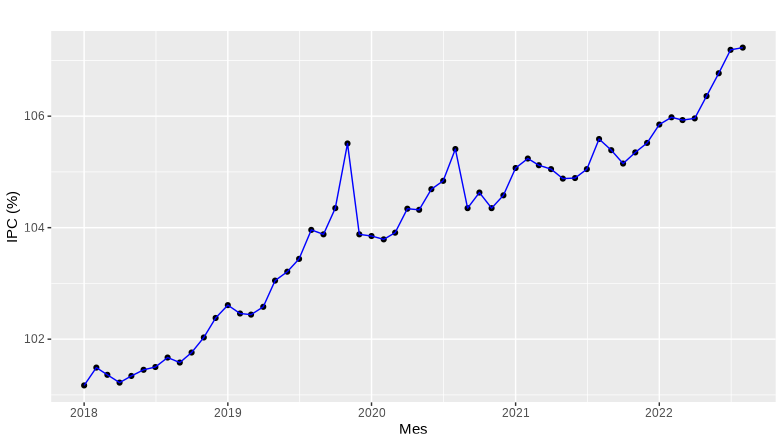
\includegraphics[width=\textwidth]{../images/histograma.png}
 % histograma.png: 868x539 px, 96dpi, 22.97x14.26 cm, bb=0 0 651 404
\end{figure}

Ejecutando el analisis en R podemos obtener la tabla:

\begin{center}
\begin{tabular}{lll}
Modelo & a & b\\
G(1,1) & -0.0009457664 & 101.3253 \\
Verhulst & 0.004454632 & 5.297622e-05 \\
Lineal & 0.003250051 & 44.355156528 \\
\end{tabular}
\end{center}

con estos datos ya se puede graficar los modelos:


\begin{figure}[htb!]
 \centering
 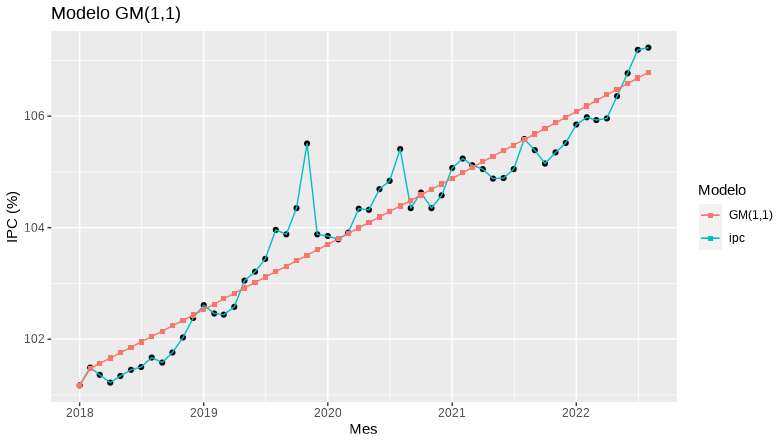
\includegraphics[width=\textwidth]{../images/gm.png}
 % histograma.png: 868x539 px, 96dpi, 22.97x14.26 cm, bb=0 0 651 404
\end{figure}

\begin{figure}[htb!]
 \centering
 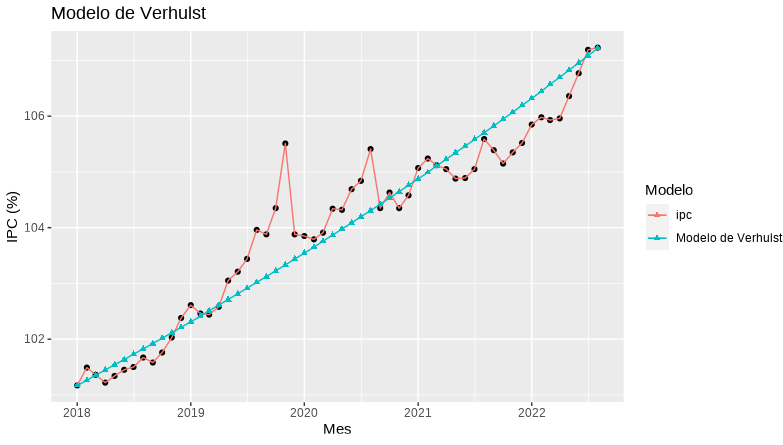
\includegraphics[width=\textwidth]{../images/ver.png}
 % histograma.png: 868x539 px, 96dpi, 22.97x14.26 cm, bb=0 0 651 404
\end{figure}

\begin{figure}[htb!]
 \centering
 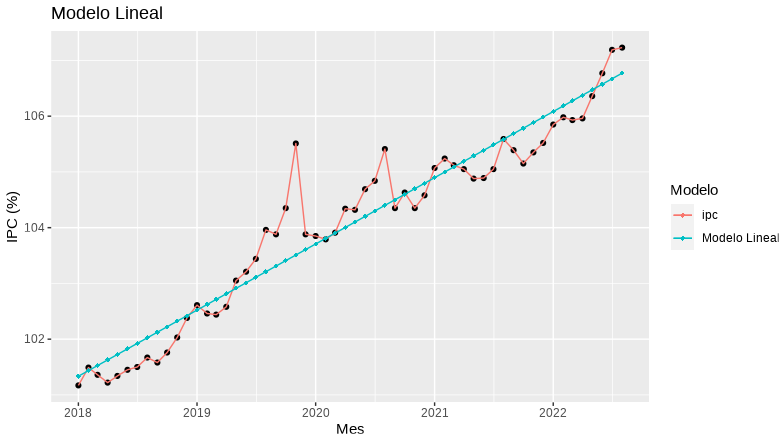
\includegraphics[height=5.5cm]{../images/lineal.png}
 % histograma.png: 868x539 px, 96dpi, 22.97x14.26 cm, bb=0 0 651 404
\end{figure}

\begin{figure}[htb!]
 \centering
 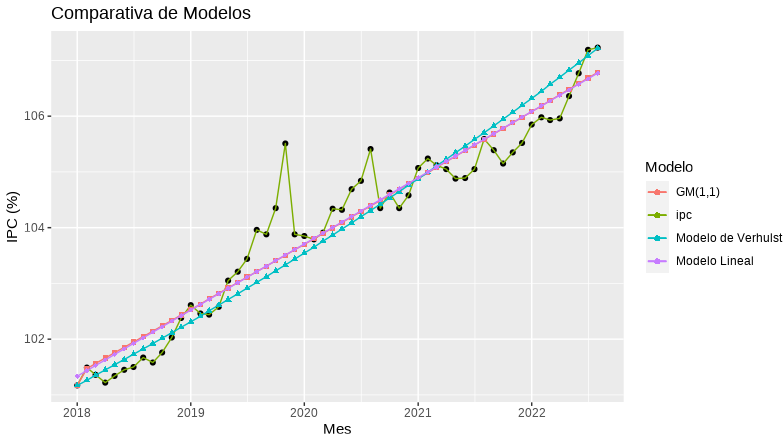
\includegraphics[width=\textwidth]{../images/comparativa.png}
 % histograma.png: 868x539 px, 96dpi, 22.97x14.26 cm, bb=0 0 651 404
\end{figure}

Ya con los modelos podemos revisar sus predicciones a 3 meses a partir de Agosto 2022

\begin{figure}[htb!]
 \centering
 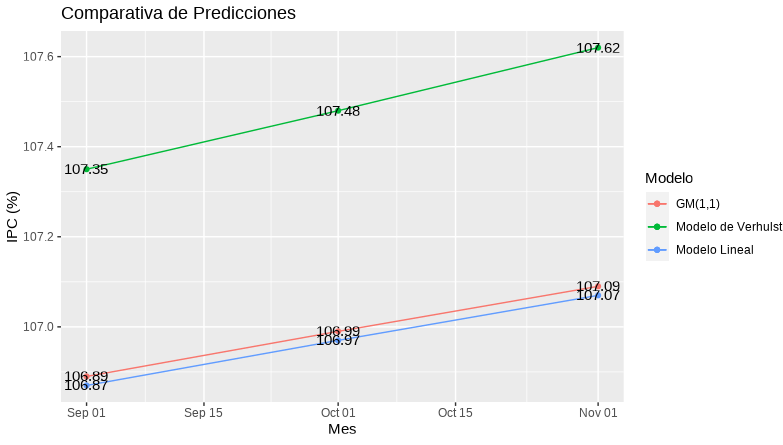
\includegraphics[width=\textwidth]{../images/pred.png}
 % histograma.png: 868x539 px, 96dpi, 22.97x14.26 cm, bb=0 0 651 404
\end{figure}

\section{Codigo de Simulacion}
El Codigo utilizado para simular los modelos y realizar los graficos es:

\begin{lstlisting}[language = R]

require(tidyverse)
require(ggplot2)
library(ggplot2)
library(tidyverse)
require("devtools")
library("devtools")
install_github("exoplanetX/greyforecasting")
library(greyforecasting)


arr <- c(101.17, 101.49, 101.36, 101.22, 101.34, 101.45, 101.5,
101.67, 101.58, 101.76, 102.03, 102.38, 102.61, 102.46, 102.44,
102.58, 103.05, 103.21, 103.44, 103.96, 103.88, 104.35, 105.51,
103.88, 103.85, 103.79, 103.91, 104.34, 104.32, 104.69, 104.84,
105.41, 104.35, 104.63, 104.35, 104.58, 105.07, 105.24, 105.12,
105.05, 104.88, 104.89, 105.05, 105.59, 105.39, 105.15, 105.35,
105.52, 105.85, 105.98, 105.93, 105.96, 106.36, 106.77, 107.19,
107.23)
d <- data_frame(
  mes = seq.Date(from = as.Date('2018-01-01'),
  to = as.Date('2022-08-01'), by = 'month'),
  ipc = arr
)

pl <- ggplot(d, mapping = aes(x=mes, y= ipc)) + labs(title = '',
  x='Mes', y='IPC (%)')
pl + geom_point() + geom_line(colour='blue')

gmo <- gm(d$ipc, term = 3)
verl <- verhulst(d$ipc, term = 3)
lin <- lm(data = d, formula = 'ipc ~ mes')

models <- data.frame(
  mes = d$mes,
  gm = gmo$fitted,
  ver = verl$fitted,
  lin = lin$fitted.values
)

plot_gm <-  pl + geom_point() + geom_line(mapping = aes(colour='ipc')) +
  geom_line(data = models, mapping = aes(mes, gm, colour = 'GM(1,1)') ) +
  geom_point(data = models, mapping = aes(mes, gm, colour = 'GM(1,1)'),
    shape = 15) +
  labs(colour = 'Modelo', title = 'Modelo GM(1,1)')

plot_ver <- pl + geom_point() + geom_line(mapping = aes(colour='ipc')) +
  geom_line(data = models, mapping = aes(mes, ver, colour = 'Modelo de Verhulst')) +
  geom_point(data = models, mapping = aes(mes, ver, colour = 'Modelo de Verhulst'),
    shape = 17) +
  labs(colour = 'Modelo', title = 'Modelo de Verhulst')

plot_lin <- pl + geom_point() + geom_line(mapping = aes(colour='ipc')) +
  geom_line(data = models, mapping = aes(mes, lin, colour = 'Modelo Lineal'),
    show.legend = TRUE) +
  geom_point(data = models, mapping = aes(mes, lin, colour = 'Modelo Lineal'),
    shape = 18) +
  labs(colour = 'Modelo', title = 'Modelo Lineal')

plot_main <- pl + geom_point() + geom_line(mapping = aes(colour='ipc')) +
  geom_line(data = models, mapping = aes(mes, gm, colour = 'GM(1,1)') ) +
  geom_point(data = models, mapping = aes(mes, gm, colour = 'GM(1,1)'),
    shape = 15) +
  geom_line(data = models, mapping = aes(mes, ver, colour = 'Modelo de Verhulst')) +
  geom_point(data = models, mapping = aes(mes, ver, colour = 'Modelo de Verhulst'),
    shape = 17) +
  geom_line(data = models, mapping = aes(mes, lin, colour = 'Modelo Lineal'),
    show.legend = TRUE) +
  geom_point(data = models, mapping = aes(mes, lin, colour = 'Modelo Lineal'),
    shape = 18) +
  labs(colour = 'Modelo', title = 'Comparativa de Modelos')

plot_gm
plot_ver
plot_lin
plot_main

new_month <- seq.Date(from = as.Date('2022-09-01'),
  to = as.Date('2022-11-01'), by = 'month')

prediction <- data.frame(
  mes = new_month,
  gm = round(gmo$forecasts,2),
  ver = round(verl$forecasts,2),
  lin = round(predict(lin, newdata = data.frame(mes = new_month)),2)
)

ggplot(prediction, mapping = aes(x = mes)) +
  geom_point(aes(y=gm, colour = 'GM(1,1)', label=gm)) +
  geom_line(aes(y=gm, colour = 'GM(1,1)')) +
  geom_point(aes(y=ver, colour = 'Modelo de Verhulst')) +
  geom_line(aes(y=ver, colour = 'Modelo de Verhulst')) +
  geom_point(aes(y=lin, colour = 'Modelo Lineal')) +
  geom_line(aes(y=lin, colour = 'Modelo Lineal')) +
  geom_text(aes(y=gm, label= gm),check_overlap = TRUE) +
  geom_text(aes(y=ver, label= ver), check_overlap = TRUE) +
  geom_text(aes(y=lin, label= lin), check_overlap = TRUE) +
  labs(colour = 'Modelo', title = 'Comparativa de Predicciones',
    x='Mes', y='IPC (%)')

\end{lstlisting}




\section{Conclusiones}

La prediiccion del \ipc debe manejarse con sumo cuidado debido a su naturaleza volatil y a su dependencia del mercado y el valor adquisitivo de la moneda, por eso se utilizo el modelo de Grey que es capaz de adaptarse a los cambios y eventos externmos que puedan influir en el valor del \ipc. Dada la situacion actual del pais con un crecimiento el modelo de Verhulst es el mejor indicador  ya que se partio de un estado de crecimiento exponencial y se espera llegar a un estado de equilibrio, pero una vez logrado el modello de Grey sera el mejor  modelo predictivo, el modelo lineal tambien parece ser un buen indicador sin embargo este no contempla  que en algun punto deje de ser posible el crecimiento del \ipc.

Por tanto para los proximos 3 meses se prevee un aumento del \ipc con los valores de 106.89, 106.99 y 107.09 [\%] en cada mes respectivamnte.

\printbibliography

\end{document}

